\section{A posteriori global-barrier certificates}\label{sec:certificate}

We give sufficient conditions whose numerical content consists of finite
matrix inequalities, scalar interval bounds, and a finite boundary ledger.
The conditions apply to the full space $\X$. Their verification does not
restrict perturbations to a symmetry class or identify a finite-box
Hessian with its infinite-lattice counterpart. Throughout this section,
$F=\nabla_\X\E$, $H_\theta=DF(\theta)$, and
$\Lambda=1/\sqrt2$ is the Hessian Lipschitz constant from
\cref{lem:basic}. The weaker bound $\Lambda=1$ may instead be used
in an individual numerical estimate when its sufficient inequalities still
hold. In particular, the correction estimates below allow that coarser
choice; the displayed cap parameters use the sharp bound, or its rational
upper bound $71/100$.
Unmarked norms and pairings are those of $\X$, with induced operator
norms; finite coordinate vectors carry their Euclidean norm.

The input representation matters. Each candidate is a specified analytic
finite-energy reference plus a compact dyadic correction. Its exterior
energy, force, branch, and edge-increment remainders must have proved
bounds. All core--exterior interface bonds are included. Finite arrays
alone do not certify a full $\X^*$ residual. The construction below is an
a posteriori criterion for such represented data, rather than an
algorithm guaranteed to succeed for every configuration.

\subsection{Full-space coercivity from finite matrices}

Let $Q:\R^d\to\X$ have linearly independent compact columns
$q_1,\ldots,q_d$, and write
\begin{equation}\label{eq:cert-projections}
 G=Q^*Q,\qquad P_Q=QG^{-1}Q^*,\qquad Y=\ker Q^*.
\end{equation}
The case $d=0$ means $Y=\X$ and no deflation. The projection is exact;
an approximate normalization of stored columns is not substituted for $G$.

\begin{lemma}[Neumann comparison]\label{lem:cert-neumann}
Let $f$ be an algebraically zero-mean vertex load supported in a square
of $N\times N$ vertices, $N\ge2$. Let $L_N$ count only bonds interior to that
square. If $f^\sharp$ denotes its Riesz representative in $\X$, then
\begin{equation}\label{eq:cert-neumann}
 \nrm{f^\sharp}^2\le f^TL_N^\dagger f,
 \qquad
 \left|f^TL_N^\dagger f-f^Tu\right|
 \le \|f\|_{\ell^2}\frac{N^2}{4}\|f-L_Nu\|_{\ell^2}
\end{equation}
for every finite proposal $u$. No mean constraint on $u$ is required.
\end{lemma}
\begin{proof}
In the variational formula
$\nrm{f^\sharp}^2=\sup_v(2f[v]-\nrm{v}^2)$, discard all bonds not
interior to the square. The supremum increases to the finite Neumann
problem. The constant mode causes no obstruction because $f$ has zero
mean. Moreover,
$\lambda_1(L_N)=4\sin^2(\pi/(2N))\ge4/N^2$.
Choose a solution $u_*$ of $L_Nu_*=f$ with the same mean as $u$.
Then $\|u_*-u\|_{\ell^2}\le N^2\|f-L_Nu\|_{\ell^2}/4$, which proves the
second inequality by pairing with $f$.
\end{proof}

The square in this lemma must contain the complete load, including both
endpoints of every nonzero flux bond used to form its divergence. The
inequality is an upper comparison; it gives no lower bound on the
infinite dual norm. Mutual load pairings can be enclosed by the same
finite solves and residual bounds. A separately proved residual
remainder $D^*r$, with $\|r\|_{\ell^2}\le\varepsilon$, contributes
at most $\varepsilon$ to the dual norm.

For the fixed neutral dipole used below, Appendix~\ref{app:reflected-residual}
proves the finite load's zero mean by compact-flux cancellation and reflection
of the analytic reference, without assuming symmetry of the saddle correction.
It also derives the explicit exterior dual remainder and includes the
core--exterior interface. Thus the mean condition in
\cref{lem:cert-neumann} is checked algebraically for these inputs.

\begin{proposition}[Deflated signed-resistance test]\label{prop:cert-gram}
Suppose, uniformly over a prescribed set of configurations,
\begin{equation}\label{eq:cert-deficits}
 H_\theta[v,v]\ge a_0\nrm{v}^2
       -\sum_{e\in S}W_e|D_ev|^2,\qquad a_0>0,\quad W_e\ge0,
\end{equation}
where $S$ is finite. A containing Neumann square includes both endpoints
of every bond in $S$ and the complete supports of $Q$, whose columns
vanish on its boundary. Let
$R_N=(f_e^TL_N^\dagger f_f)_{e,f\in S}$, where
$f_e=\delta_{e^+}-\delta_{e^-}$, and let $B_{ej}=D_eq_j$.
If the finite matrix inequality
\begin{equation}\label{eq:cert-matrix-test}
 W^{1/2}(R_N-BG^{-1}B^T)W^{1/2}
       \preceq a_0\kappa I,\qquad \kappa<1,
\end{equation}
is verified, then $H_\theta|_Y\succeq\mu I$ on the full infinite
complement, where $\mu=a_0(1-\kappa)>0$.
\end{proposition}
\begin{proof}
The infinite trace Gramian restricted to $Y$ is
$R_\infty^Y=R_\infty-BG^{-1}B^T$. Applying
\cref{lem:cert-neumann} to every linear combination of the loads gives
$R_\infty\preceq R_N$. Thus the norm squared of the weighted trace
map $v\mapsto (\sqrt{W_e}D_ev)_{e\in S}$ on $Y$ is at most
$a_0\kappa$. Substitution in \eqref{eq:cert-deficits} proves the claim.
The zero boundary values of the reaction columns ensure that their
finite and infinite energy products agree.
\end{proof}

The test uses the entire matrix, including mutual resistances. A
validated congruence using interval enclosures of all its entries is
sufficient. Individual diagonal resistance tests are not equivalent.
Finite signed-Laplacian reductions have substantial precedents
\cite{Chen2020}; the role of \cref{prop:cert-gram} here is to preserve
the direction of the comparison with the infinite complement.

The weights in \eqref{eq:cert-deficits} are obtained from interval
enclosures of $\cos(D_e\theta)$, with an analytic positive floor outside
$S$. For a chart displacement $w\in Y$, $\nrm{w}\le R$, the sharper
edge estimate
\begin{equation}\label{eq:cert-deflated-edge}
 |D_ew|\le R\sqrt{\tfrac12-b_e^TG^{-1}b_e},
 \qquad b_e=(D_eq_1,\ldots,D_eq_d)^T,
\end{equation}
follows by subtracting the projection of the edge evaluation functional.
It is used before enclosing the trigonometric weights. Negative core
bonds are allowed; positivity is required of the resulting form.

\subsection{Critical points and exact saddle planes}

\begin{lemma}[Frozen Newton and Morse index]\label{lem:cert-newton}
Let $\widehat\theta\in\X$ and $\nrm{F(\widehat\theta)}\le\delta$.
Assume either $H_{\widehat\theta}\succeq\gamma I>0$, or there is a unit
$q\in\X$ such that
\begin{equation}\label{eq:cert-saddle-splitting}
 H_{\widehat\theta}[q,q]\le-a<0,\qquad
 H_{\widehat\theta}|_{q^\perp}\succeq c_{\perp}I>0,
 \qquad \gamma=\min(a,c_{\perp}).
\end{equation}
If
\begin{equation}\label{eq:cert-newton-radius}
 \delta+\tfrac\Lambda2\rho^2\le\gamma\rho,
 \qquad \Lambda\rho<\gamma,
\end{equation}
there is a unique critical point $\theta_*$ in
$\overline B_\X(\widehat\theta,\rho)
 =\{u:\nrm{u-\widehat\theta}_\X\le\rho\}$. It is a strict minimum in the
first case and has Morse index one in the second. Its Hessian inverse
has norm at most $(\gamma-\Lambda\rho)^{-1}$.
\end{lemma}
\begin{proof}
In the saddle case write $v=tq+y$ and set $Jv=-tq+y$. Self-adjointness
cancels the cross terms:
\[
 \inner{H_{\widehat\theta}v}{Jv}
 =-t^2H_{\widehat\theta}[q,q]+H_{\widehat\theta}[y,y]
 \ge\gamma\nrm{v}^2.
\]
Lax--Milgram applied to $JH_{\widehat\theta}$ gives an inverse bounded
by $1/\gamma$. The positive $q^\perp$ block has a negative scalar
Schur complement, so its Morse index is exactly one. No smallness
assumption on the off-diagonal block is needed. In the minimum case
the inverse bound is immediate. The map
$h\mapsto-H_{\widehat\theta}^{-1}(F(\widehat\theta)+\mathcal N(h))$
is a self-map and contraction on the closed radius-$\rho$ ball by
$\nrm{\mathcal N(h)}\le\Lambda\nrm{h}^2/2$ and
$\operatorname{Lip}(\mathcal N)\le\Lambda\rho$.
This closed ball is complete. If the first inequality in
\eqref{eq:cert-newton-radius} is strict, the fixed point is also in the
open ball.
The same diagonal signs persist throughout that ball, proving the
index and inverse bounds at the exact critical point.
\end{proof}

The positive blocks in this lemma can be certified by
\cref{prop:cert-gram}, with zero or one deflated direction. This is a
validation criterion for supplied candidates, not a search or
classification of all critical points; compare finite XY certification
in \cite{Mehta2014}. Coercivity of an isolated configuration and
superposition arguments also have prior uses in lattice models
\cite{Hudson2015}.

Useful energy and charge consequences are
\begin{equation}\label{eq:cert-critical-energy}
 |\E(\theta_*)-\E(\widehat\theta)|
 \le\min\left\{\frac{\rho^2}{2},
               \frac{\delta\rho}{2}+\frac{\Lambda\rho^3}{12}\right\}.
\end{equation}
For the second bound apply stationary-endpoint quadrature to
$g(t)=\E(\widehat\theta+t(\theta_*-\widehat\theta))$:
$g'(1)=0$ and
$g(1)-g(0)-g'(0)/2=\int_0^1(1/2-t)g''(t)\,dt$.
Subtract $g''(1/2)$ in the integral. A global branch margin greater than
$\rho/\sqrt2$ preserves all plaquette charges under the correction.
At a minimum the correction segment is convex, so its energy never
exceeds $\E(\widehat\theta)$.

An optimal-height separator needs planes through the exact saddle.
For a saddle $s$ validated near $\widehat s$, let $q$ be its certified
candidate direction, and put
\[
 \sigma=\nrm{P_Qq}>0,\qquad r=P_Qq/\sigma,
 \qquad \delta_Q=\sqrt{1-\sigma^2}<1/\sqrt2.
\]
Choose $A_0\ge-H_{\widehat s}[q,q]$ and
$\eta_0\ge\nrm{P_{q^\perp}H_{\widehat s}q}$.

\begin{lemma}[Projected cap and adjoint offset]\label{lem:cert-cap}
Suppose the candidate complement floor is $c_{\perp}$ and
\begin{equation}\label{eq:cert-cap-coercivity}
 \mu=c_{\perp}(1-\delta_Q^2)-2\eta_0\delta_Q\sqrt{1-\delta_Q^2}
               -A_0\delta_Q^2-\Lambda\rho_s>0.
\end{equation}
Then $H_s|_{r^\perp}\succeq\mu I$. For $0<R_c<3\mu/\Lambda$,
\begin{equation}\label{eq:cert-cap-energy}
 \E(s+h)\ge\E(s)+k_c\nrm{h}^2,
 \quad h\perp r,\quad\nrm{h}\le R_c,
 \qquad k_c=\frac\mu2-\frac{\Lambda R_c}{6}>0.
\end{equation}
For any adjoint proposal $z$ with
$\nrm{H_{\widehat s}z-r}\le\eta_z$,
\begin{equation}\label{eq:cert-adjoint-offset}
 \left|\inner{r}{s-\widehat s}+\inner{F(\widehat s)}{z}\right|
 \le\eta_z\rho_s+\tfrac12\|Dz\|_{\ell^\infty}\rho_s^2.
\end{equation}
\end{lemma}
\begin{proof}
For unit $h\perp r$ write $h=tq+y$, where $|t|\le\delta_Q$ and
$\nrm{y}=\sqrt{1-t^2}$. Its candidate quadratic form is bounded below
by $c_{\perp}(1-t^2)-2\eta_0|t|\sqrt{1-t^2}-A_0t^2$.
This expression is nonincreasing for $0\le|t|\le\delta_Q<1/\sqrt2$.
Evaluate it at $\delta_Q$ and subtract $\Lambda\rho_s$ once at operator
level. Taylor's theorem at the stationary point $s$ proves
\eqref{eq:cert-cap-energy}. To prove \eqref{eq:cert-adjoint-offset},
test $F(\widehat s)+H_{\widehat s}(s-\widehat s)+\mathcal N=0$ against
$z$. The scalar sine remainder gives
$|\inner{\mathcal N}{z}|\le\|Dz\|_{\ell^\infty}\rho_s^2/2$.
\end{proof}

With $a(\theta)=G^{-1}Q^*(\theta-\theta_{\rm ref})$, the exact plane is
\begin{equation}\label{eq:cert-exact-plane}
 \ell(\theta)=\inner{r}{\theta-s}=n^Ta(\theta)-d=0,
 \qquad n=Q^*r,\quad d=\inner{r}{s-\theta_{\rm ref}}.
\end{equation}
The adjoint bound encloses $d$ by computable loads and residuals. An
interval strip covering this plane is used to test its intersections;
the separator itself is cut by the exact plane, not an approximate
midpoint plane. A plane through $\widehat s$ generally has a nonzero
linear energy term and does not establish an exact saddle-height barrier.

\subsection{Entire fibers and the boundary ledger}

Let $A_i\subset\R^d$ be finitely many bounded open coordinate domains,
$y_i\in Y$, and $R_i>0$. Define
\begin{equation}\label{eq:cert-atlas}
 c_i(a)=\theta_{\rm ref}+Qa+y_i,\qquad
 U_i=\{c_i(a)+w:a\in A_i,\ w\in Y,\ \nrm{w}<R_i\}.
\end{equation}
Let $A_0$ be a bounded open coordinate disk or polytope and set
$D_0=(\bigcup_iU_i)\cap a^{-1}(A_0)$.
For a common exact reference energy $e_{\rm ref}$, suppose the chart
oracles give, on their complete closed parameter cells,
\begin{equation}\label{eq:cert-fiber-oracle}
 H_{c_i(a)+w}|_Y\succeq\mu_i I>0\quad(\nrm{w}\le R_i),
 \quad\nrm{P_YF(c_i(a))}\le\beta_i(a),
 \quad\E(c_i(a))-e_{\rm ref}\ge V_i^-(a).
\end{equation}
Consequently
\begin{equation}\label{eq:cert-fiber-parabola}
 \E(c_i(a)+w)-e_{\rm ref}
 \ge V_i^-(a)-\beta_i(a)\nrm{w}+\tfrac12\mu_i\nrm{w}^2.
\end{equation}
The reference may remain symbolic: relative-energy bounds between
compact changes of the same analytic background avoid subtracting broad,
unrelated absolute-energy intervals.

\begin{lemma}[Fiber minimization and cap lifting]\label{lem:cert-fiber}
If $\beta_i(a)<\mu_iR_i$, the fiber has a unique interior minimizer
$w_i(a)$ with $\nrm{w_i(a)}\le\beta_i(a)/\mu_i$. Suppose $a$ is on
the exact plane of a saddle satisfying \cref{lem:cert-cap}, and
\begin{equation}\label{eq:cert-cap-lifting}
 \nrm{c_i(a)-\widehat s}+\rho_s+\frac{\beta_i(a)}{\mu_i}<R_c.
\end{equation}
Then every $w\in Y$, $\nrm{w}\le R_i$, satisfies
\begin{equation}\label{eq:cert-full-fiber-cap}
 \E(c_i(a)+w)\ge\E(s)
  +k_c\nrm{c_i(a)+w_i(a)-s}^2
  +\tfrac12\mu_i\nrm{w-w_i(a)}^2.
\end{equation}
\end{lemma}
\begin{proof}
Strong convexity on the closed Hilbert ball gives weak lower
semicontinuity after extending the function by $+\infty$ outside the
ball. Weak compactness gives a minimizer. On its boundary the radial
derivative is at least $\mu_iR_i^2-\beta_i(a)R_i>0$, excluding a
boundary minimizer. Strong monotonicity proves uniqueness and the norm
bound. Since $r\in\operatorname{ran}Q$, every $w\in Y$ is orthogonal
to $r$. Thus the minimizing point remains in the exact saddle plane;
\eqref{eq:cert-cap-lifting} puts it inside the cap. Apply
\eqref{eq:cert-cap-energy} there and strong convexity from that point
to $w$.
\end{proof}

It is the minimizing point that must fit in the cap, not the entire
transverse ball. In verifying \eqref{eq:cert-cap-lifting}, retain the
orthogonal decomposition
\[
 \nrm{c_i(a)-\widehat s}^2
 =(a-\widehat a_s)^TG(a-\widehat a_s)
   +\nrm{y_i-P_Y(\widehat s-\theta_{\rm ref})}^2.
\]
No global identification of minimizers belonging to different charts
is needed for these energy inequalities.

\begin{figure}[t]
\centering
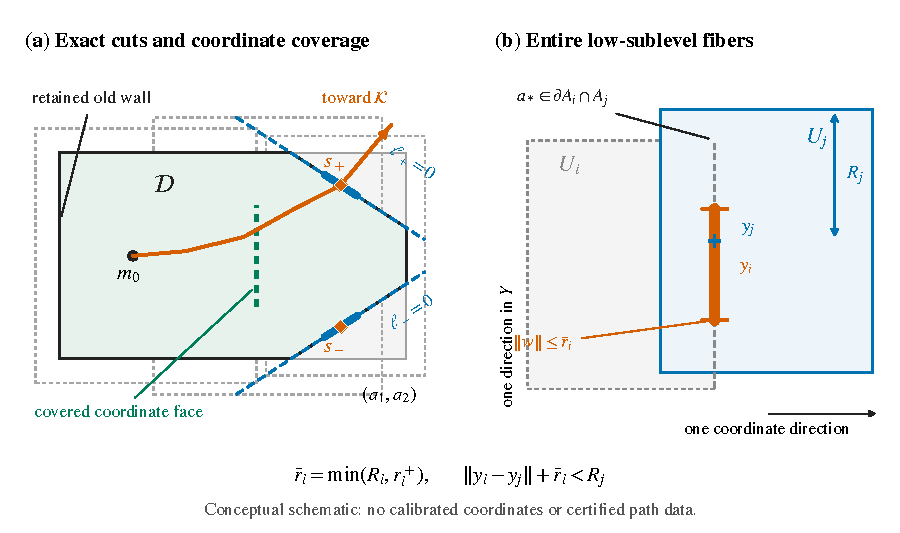
\includegraphics[width=\linewidth]{figures/certificate_geometry.pdf}
\caption{Conceptual certificate geometry; positions and proportions are
not numerical atlas data or a computed orbit. (a) Reaction coordinates,
with transverse fibers suppressed. The exact cuts pass through $s_\pm$;
thick blue segments depict local cap sections. A covered coordinate face
is internal, while a retained old wall needs an energy bound. The orange
line sketches the upper construction through $s_+$. (b) One coordinate
direction and one illustrative direction in $Y$. The entire permitted
low-sublevel fiber ball must lie strictly inside the neighboring chart,
with the complete coordinate cell inside $A_j$. The displayed Hilbert-norm
inequality, rather than overlap in this drawn slice, certifies inclusion
in every transverse direction.}
\label{fig:certificate-geometry}
% ALT TEXT: Two conceptual panels show the separating atlas. The left
% panel has overlapping coordinate rectangles, a minimum, two exact cuts
% through the saddles, a covered coordinate face, a retained outer wall,
% and an illustrative upper path. The right panel shows the complete
% allowed low-energy transverse interval inside a neighboring fiber ball.
% This interval is only a slice of the infinite-dimensional ball; the
% displayed norm inequality certifies full inclusion. No coordinates in
% the figure are calibrated certificate data.
\end{figure}

\Cref{fig:certificate-geometry} separates the local cap and chart-coverage
obligations. Because each normal lies in $\operatorname{ran}Q$, its exact
cut is constant along the $Y$ fibers. The cap bounds the fiber minimizer;
strong convexity then controls all other fiber points. Coverage of a
coordinate face instead uses inclusion of its whole possible low-energy
fiber ball, as quantified below.

For clarity, we describe the finite boundary tests. Let $h$ be the exact
level to be certified and $\overline h\ge h-e_{\rm ref}$ a verified
upper enclosure of its relative energy. Subdivide complete closed faces and intersections, including
their edges and corners. Each retained cell receives one of the
following witnesses.
\begin{enumerate}
\item A radial wall of chart $i$ passes if
\begin{equation}\label{eq:cert-radial-test}
 V_i^- -\beta_iR_i+\tfrac12\mu_iR_i^2\ge \overline h.
\end{equation}
\item Any full-fiber piece passes directly if
$V_i^--\beta_i^2/(2\mu_i)\ge \overline h$.
Otherwise put
\[
 \Delta_i=\beta_i^2+2\mu_i(\overline h-V_i^-),\qquad
 r_i^+=\frac{\beta_i+\sqrt{\Delta_i}}{\mu_i}
\]
when $\Delta_i\ge0$. A negative $\Delta_i$ excludes the sublevel.
Every point with $\E<h$ has $\nrm{w}<r_i^+$. A coordinate-face cell
is therefore internal if a chart $j$ contains its complete coordinate
cell strictly and
\begin{equation}\label{eq:cert-overlap-test}
 \nrm{y_i-y_j}+\min(R_i,r_i^+)<R_j.
\end{equation}
The stronger full-ball test replaces the minimum by $R_i$.
To prove that a point is internal to $D_0$, the coordinate cell must also
lie in $A_0$. Chart overlap alone cannot make a point on the outer
coordinate boundary internal to $D_0$.
\item A new exact-plane face passes by
\cref{lem:cert-fiber}, uniformly over its intersection with the closed
chart, coordinate region, and other cuts. Computations may overcover
the plane by the interval strip from \eqref{eq:cert-adjoint-offset}.
\item Near a cap, a retained outer boundary or seam can instead use
the following scalar cone bound. If
$H_s[r,r]\ge-A$ and
$\nrm{P_{r^\perp}H_sr}\le\kappa_r$, write
$\theta-s=tr+v$, $v\perp r$. Given
$|t|\le T$, $\nrm{v}\in[y_-,y_+]$ and
$\nrm{\theta-s}\le H_0$, set
\[
 p=\frac\mu2-\frac{\Lambda H_0}{6}>0,\quad
 q_c=\frac A2+\frac{\Lambda H_0}{6},\quad
 y_* =\operatorname{clamp}\left(\frac{\kappa_rT}{2p},y_-,y_+\right).
\]
Then the test
\begin{equation}\label{eq:cert-cone-test}
 p y_*^2-\kappa_rT y_*-q_cT^2\ge0
\end{equation}
implies $\E(\theta)\ge\E(s)$ throughout the piece. Indeed Taylor's
lower bound is
$\mu\nrm{v}^2/2-\kappa_r|t|\nrm{v}-At^2/2
-\Lambda(t^2+\nrm{v}^2)^{3/2}/6$; replacing the last square root by
$H_0$ leaves the displayed quadratic minimum.
\end{enumerate}

All quantities in these tests have interval enclosures obtained from
Gram matrices, finite loads, and the specified analytic remainders.
A boundary ledger records a complete finite closed cover and the test
used on each cell. Pairwise intersections of chart balls, a mesh of
boundary samples, or a list omitting tangencies do not establish
coverage. In particular the outer coordinate circle is checked as a
continuum. The ledger does not assert that a failed test exhibits an
actual lower-energy escape.

To make retention by the exact saddle cuts explicit, write
\[
 H_{\rm cl}=\bigcap_j\{\ell_j\le0\},\qquad
 H_{\rm op}=\bigcap_j\{\ell_j<0\},\qquad D=D_0\cap H_{\rm op}.
\]
For each closed old-wall cell $C_\alpha$, the retained set is
$C_\alpha\cap H_{\rm cl}$. The set-level obligation is
\[
 \theta\in C_\alpha\cap H_{\rm cl},\quad\E(\theta)<h
       \quad\Longrightarrow\quad\theta\in D_0.
\]
An energy bound proves this implication vacuously; a full-fiber overlap
witness proves it by strict inclusion in $D_0$. A cell may be discarded
by cuts after verifying $C_\alpha\cap H_{\rm cl}=\varnothing$.
Strict positivity of one cut throughout the cell is sufficient but not
necessary: a rigorous joint infeasibility test may also establish this.
Equality at a cut is retained whenever all other closed inequalities
hold. Exclusion from $H_{\rm op}$ alone does not justify discarding a
tangency or an old-wall/new-plane intersection.

Membership and target exclusion are additional finite tests. The entire
minimum enclosure must lie strictly inside a chart, the coordinate
region, and every retained halfspace. A useful sufficient exclusion is
\begin{equation}\label{eq:cert-vacuum-exclusion}
 \sup_{\theta\in\overline D_0}\nrm{\theta-m}<2,
\end{equation}
when $m$ has a certified charged plaquette. The four principal increments
on that plaquette imply $\E(m)\ge2$. For every $k\in\K$,
$\E(m)=\E(m-k)\le\nrm{m-k}^2/2$, so
$\operatorname{dist}_\X(m,\K)\ge2$.
The supremum in \eqref{eq:cert-vacuum-exclusion} is bounded using the
finite coordinate region, $G$, the chart centers and radii, and the
minimum enclosure. Alternatively one may certify charge preservation
throughout the closed atlas. Discreteness of $\K$ alone does not locate
the atlas relative to all its nonzero lifts.

\subsection{Upper paths attached to exact critical points}

For explicit consecutive nodes $u_j,u_{j+1}\in\X$, the global bound
$\nrm{H_\theta}\le1$ gives
\begin{equation}\label{eq:cert-segment-test}
 \max_{0\le t\le1}\E((1-t)u_j+tu_{j+1})
 \le\max\{\E(u_j),\E(u_{j+1})\}
             +\tfrac18\nrm{u_{j+1}-u_j}^2.
\end{equation}
This checks the entire time segment. The nodes use coherent real lifts;
independent choices of principal phases at successive times do not
automatically define an $\X$-continuous path.

\begin{lemma}[Stationary-endpoint attachment]\label{lem:cert-hermite}
Let $s$ be exact and stationary, $\nrm{s-\widehat s}\le\rho_s$, and
$|\E(s)-\E(\widehat s)|\le\varepsilon_s$. For an explicit node $c$,
suppose $d_c\ge\nrm{c-\widehat s}$ and
$\Delta_c^+\ge\E(c)-\E(\widehat s)$. If
\begin{equation}\label{eq:cert-hermite-test}
 \Delta_c^++\varepsilon_s+\frac\Lambda6(d_c+\rho_s)^3<0,
\end{equation}
the segment from $s$ to $c$, except at $s$, has energy strictly below
$\E(s)$.
\end{lemma}
\begin{proof}
For $g(t)=\E(s+t(c-s))$, one has $g'(0)=0$ and
$|g'''|\le\Lambda(d_c+\rho_s)^3$. Stationary-endpoint Hermite
interpolation yields
\[
 g(t)\le(1-t^2)\E(s)+t^2\E(c)
       +\frac\Lambda6(d_c+\rho_s)^3t^2(1-t).
\]
The test makes the difference from $\E(s)$ strictly negative for $t>0$.
\end{proof}

Thus no constant energy penalty proportional to $\rho_s^2$ is paid near
the saddle. Two attachment nodes enter opposite local descending sides
if their $q$-coordinates relative to $\widehat s$ have opposite signs
and absolute values greater than $\rho_s$. The positive transverse
block and negative Schur complement identify the two local strict
sublevel components. These are variational attachments, not validated
heteroclinic orbits; rigorous transition-path validation has its own
antecedents and additional obligations \cite{Breden2019}.

The minimum is attached to its candidate by the convex bridge from
\cref{lem:cert-newton}. Polygonal arms strictly below $\E(s)$ and two
tests \eqref{eq:cert-hermite-test} then connect that exact minimum through
$s$ to a terminal configuration. To reach the physical target, certify
zero charge on every terminal plaquette, including the analytic
exterior. If $\beta_e\in(-\pi,\pi]$ are its principal increments, then
$(D_e\theta-\beta_e)/(2\pi)$ is a curl-free integer bond field of finite
support. Integrating it gives a compact integer function $n$, after
subtracting its exterior constant. Hence
$\theta=2\pi n+\eta$ with $D\eta=\beta$, and
\begin{equation}\label{eq:cert-terminal-path}
 \theta(t)=2\pi n+(1-t)\eta
\end{equation}
has nonincreasing energy and ends in $\K$. The finite support follows
because a nonzero integer slip requires $|D_e\theta|\ge\pi$, and
$D\theta\in\ell^2$. Summability and domination justify continuity and
monotonicity of the infinite sum. A finite core check discharges this
condition only together with exterior branch and interface checks.
The terminal real lift need not be zero; a claim about that particular
representative requires the additional verification $n=0$.

\subsection{Global closure and reusable conditions}

\begin{theorem}[A posteriori global-barrier certificate]\label{thm:certificate}
Suppose the preceding tests validate a minimum $m$ and finitely many
index-one saddles $s_1,\ldots,s_J$. For each saddle choose a cap normal
$r_j\in\operatorname{ran}Q$ satisfying
\cref{lem:cert-cap}, and write
$\ell_j(\theta)=\inner{r_j}{\theta-s_j}$.
Fix a distinguished saddle $s_0$ and put $h=\E(s_0)$. Assume the finite
input certificate verifies the following conditions.
\begin{enumerate}
\item The exact minimum enclosure is strictly inside
$D=D_0\cap\bigcap_j\{\ell_j<0\}$, and
$\overline D_0\cap\K=\varnothing$.
\item A complete closed-cell ledger for every retained old radial,
exposed coordinate, and outer-coordinate boundary piece verifies
\eqref{eq:cert-radial-test}, the direct full-fiber bound,
\eqref{eq:cert-overlap-test}, or \eqref{eq:cert-cone-test} at level $h$.
Cells removed by another cut need not pass an energy test; their removal
must itself be verified on the complete closed cell relative to
$H_{\rm cl}$. Each retained point of energy below $h$ must be certified
strictly internal to $D_0$ by a valid coverage witness. All intersections,
edges, corners, and tangencies are included.
\item Every new face
\[
 \{\theta\in\overline D_0:\ell_j(\theta)=0,
                         \ \ell_k(\theta)\le0\ (k\ne j)\}
\]
is covered by \eqref{eq:cert-cap-lifting} and
\cref{lem:cert-fiber}, or a direct energy bound at level $h$.
For every cap used at its own saddle level, $\E(s_j)\ge h$ is certified.
\item The segment, stationary-endpoint, minimum-bridge, and terminal-lift
tests construct a path from $m$ to $\K$ with maximum $h$ through $s_0$.
\end{enumerate}
Then, over all continuous strong-$\X$ paths to the physical uniform
states,
\begin{equation}\label{eq:cert-global-identity}
 \inf_{\substack{\gamma\in C([0,1];\X)\\
        \gamma(0)=m,\ \gamma(1)\in\K}}
 \max_t\bigl(\E(\gamma(t))-\E(m)\bigr)
       =h-\E(m).
\end{equation}
\end{theorem}
\begin{proof}
The earlier tests establish exact critical points, the full-space
positive complements, and the exact cap inequalities. For a finite
union, $\partial(\bigcup_i U_i)\subset\bigcup_i\partial U_i$.
After intersecting with $a^{-1}(A_0)$ and the saddle halfspaces,
\[
 \partial D\subset
 (\partial D_0\cap H_{\rm cl})\ \cup\
 \bigcup_j(D_0\cap H_{\rm cl}\cap\{\ell_j=0\}).
\]
Indeed, every boundary point lies in $\overline D_0\cap H_{\rm cl}$;
if it is in $D_0$ and every cut is strict, it is an interior point of
$D$, a contradiction. Thus every boundary point belongs to a retained
old wall or a new plane face, including their intersections. On a coordinate wall the overlap test
places every hypothetical point below $h$ strictly inside another
chart and inside $a^{-1}(A_0)$, so it cannot belong to this boundary. All other ledger witnesses
give energy at least $h$. Hence $\E\ge h$ throughout $\partial D$.
The domain is open, contains $m$, and excludes every endpoint in $\K$.
Every admissible path has a first exit and crosses $\partial D$;
its maximum is therefore at least $h$. The validated upper path gives
the reverse inequality. No compactness of $\partial D$, attainment of
the path infimum, or invariant reduced manifold is assumed.
\end{proof}

The energy ordering in the third condition is a real obligation.
An exact symmetry preserving the energy and compatible with uniqueness
of the validated root can prove equality between reflected saddles.
Overlapping numerical energy intervals alone cannot do so.

\begin{corollary}[Several competing saddles]\label{cor:cert-competing}
If an upper path is certified through each $s_j$, and every retained
old wall is bounded below by $\min_j\E(s_j)$, then the same construction
gives barrier $\min_j\E(s_j)-\E(m)$.
\end{corollary}
\begin{proof}
Each cap is bounded below by its own saddle energy and thus by the
finite minimum. Choose a saddle attaining that minimum for the upper
path. The proof of \cref{thm:certificate} applies without determining in advance
which saddle attains the minimum.
\end{proof}

For ledger computations a direct bound by $\min_j\overline h_j$ suffices, where
$\overline h_j\ge\E(s_j)-e_{\rm ref}$ are verified relative-energy bounds. A change of
dominant mechanism requires an additional certified ordering or crossing
argument; uncertainty overlap is not evidence of a crossing. Reuse of
the theorem means verifying the same types of obligations on new data.
It does not retain old residuals, deficient-bond sets, matrix margins,
or boundary coverage automatically when the configuration changes.
